\documentclass[11pt]{article} % For LaTeX2e
\usepackage{rldmsubmit,palatino}
\usepackage{apacite}
\usepackage{color}
\usepackage{graphicx}
\usepackage{subcaption}
\usepackage{wrapfig}
\usepackage{placeins}
\usepackage{amsmath}
\usepackage{breqn}
\usepackage{units}
\usepackage{floatrow}


\definecolor{Green}{RGB}{58, 147, 48}
\newcommand{\fl}[1]{\textcolor{red}{\textsc{[#1 -Falk]}}}
\newcommand{\pmk}[1]{\textcolor{blue}{\textsc{[#1 -Paul]}}}
\newcommand{\fc}[1]{\textcolor{Green}{\textsc{[#1 -Fred]}}}

\title{Mouselab-MDP: A new paradigm for tracing how people plan}


\author{
Frederick Callaway \textsuperscript{\scriptsize 1}\\
Dept. of Psychology, UC Berkeley\\
\texttt{fredcallaway@berkeley.edu} \\
\And
Falk Lieder \textsuperscript{\scriptsize 1} \\
Dept. of Psychology, UC Berkeley \\
\texttt{falk.lieder@berkeley.edu} \\
\And
Paul M. Krueger \textsuperscript{\scriptsize 1}\\
Dept. of Psychology, UC Berkeley \\
\texttt{pmk@berkeley.edu} \\
\And
Thomas L. Griffiths \\
Dept. of Psychology, UC Berkeley\\
\texttt{tom\_griffiths@berkeley.edu}
\AND
    {\centering { \large \bf \textsuperscript{\scriptsize 1}} {\small These authors contributed equally.}}
}

% The \author macro works with any number of authors. There are two commands
% used to separate the names and addresses of multiple authors: \And and \AND.
%
% Using \And between authors leaves it to \LaTeX{} to determine where to break
% the lines. Using \AND forces a linebreak at that point. So, if \LaTeX{}
% puts 3 of 4 authors names on the first line, and the last on the second
% line, try using \AND instead of \And before the third author name.

\newcommand{\fix}{\marginpar{FIX}}
\newcommand{\new}{\marginpar{NEW}}

\begin{document}

\maketitle

\begin{abstract}

%Background and Motivation
Planning is a latent cognitive process that cannot be observed directly. This makes it difficult to study how people plan. 
%Contribution
To address this problem, we propose a new paradigm for studying planning that provides experimenters with a timecourse of participant attention to information in the task environment. This paradigm employs the information-acquisition mechanism of the Mouselab paradigm, in which participants click on options to reveal the outcome of choosing those options. However, in contrast to the original Mouselab paradigm, our paradigm is a sequential decision process, in which participants must plan multiple steps ahead to achieve high scores. We release Mouselab-MDP open-source as a plugin for the JsPsych online Psychology experiment library. The plugin displays a Markov decision process as a directed graph, which the participant navigates to maximize reward. To  trace the the process of planning, the rewards associated with states or actions are initially occluded; the participant has to click on a transition to reveal its reward. This information gathering behavior makes explicit the states the participant considers. We illustrate the utility of the Mouselab-MDP paradigm with a proof-of-concept experiment in which we trace the temporal dynamics of planning in a simple environment. Our data shed new light on people's approximate planning strategies and on how people prune decision trees.
%Conclusion
We hope that the release of Mouselab-MDP will facilitate future research on human planning strategies. In particular, we hope that the fine-grained time course data that the paradigm generates will be instrumental in specifying algorithms, tracking learning trajectories, and characterizing individual differences in human planning.
% We hope that our paradigm will facilitate reverse-engineering people's highly efficient planning algorithms, studying how planning strategies are learned and improved based on experience, and characterizing individual differences in planning strategies. 


%%%% PREVIOUS
% %Background and Motivation
% Planning is a latent cognitive process that cannot be observed directly. This makes it difficult to study how people plan. 
% %Contribution
% To address this problem, we extend an established methodology for tracing the process by which people choose between gambles to the domain of planning. We present a new plug-in for the widely used JsPsych library for programming psychology experiments \cite{DeLeeuw2015} that makes it very easy to create to create a wide range of experiments for tracing how people plan. Our Mouselab-MDP plug-in renders the Markov decision processes specified as spatial environments where each location contains a reward and the participant's task is to find the path that gathers the largest amount of reward possible. To trace the the process of planning all rewards are initially occluded and the participant has to click on a transition to reveal its reward. In this way, the paradigm records which state-transitions that participant considers during planning, when they consider them, and in which order.
% We illustrate the utility of the Mouselab-MDP paradigm with a proof-of-concept experiment in which we trace the temporal dynamics of planning in a simple environment. Our data shed new light on people's approximate planning strategies and shed new light on how people prune decision trees.
% %Conclusion
% We hope that our paradigm will facilitate reverse-engineering people's highly efficient planning algorithms, studying how planning strategies are learned and improved based on experience, and characterizing individual differences in planning strategies.
%%%%

\end{abstract}

\keywords{
planning; process tracing; meta-decision making; pruning; research methods
}

\acknowledgements{This work was supported by grant number ONR MURI N00014-13-1-0341 and a grant from the Templeton World Charity Foundation.}  


\startmain % to start the main 1-4 pages of the submission.

\section{Introduction and Background}
Many if not all of us have found ourselves in an unfortunate predicament due to a lapse of forethought. However, despite the ease with which such events come to memory, they are the exception rather than the rule. Humans have an exceptional ability to establish long-term goals and make steady progress towards their completion, often over the course of years or decades. This is only possible through planning. Planing is a broad notion, potentially taking multiple forms \cite{Morris2004}; however for present purposes, we define planning as explicitly considering potential future states, the actions one might take in them, the states that might result from those actions, and so on. For example, a student deciding whether or not to attend a class, is engaged in planning when they consider doing homework during class time and skimming the slides on the morning of the following lecture.

Planning is a fundamental aspect of higher-order cognition, and it has accordingly received much attention in cognitive psychology. Planning has been studied with verbal protocol analysis and computer simulation of problem solving \cite{NewellSimon1972}, models of the hierarchical structure of human behavior \cite{Miller1986,Botvinick2009}, errors and reaction times in sequential decision-making \cite<e.g., >{Huys2012,Huys2015}, and neural activity in spatial navigation tasks \cite{Olafsdottir2015, SimonDaw2011, Balaguer2016}. Planning has also received considerable attention in artificial intelligence \cite{Russell2010,Lavalle2006}, and Markov decision processes \cite{Sutton1998} have emerged as a common mathematical framework for bridging these two literatures.

Research on planning is complicated by the fact that we cannot directly observe the cognitive processes of planning. Thus, researchers must infer this latent cognitive process based on the decisions participants ultimately make, or on neural data which are challenging to collect and interpret. One approach to this problem is to design \emph{process tracing} paradigms that externalize some aspect of the cognitive process. \citeA{Payne1988} developed one such methodology for studying multi-alternative risky choice: the ``Mouselab'' paradigm. The paradigm presents a decision problem as a payoff matrix whose entries are initially occluded. Participants choose between multiple gambles whose outcome-dependent payoffs are recorded in the cells of the payoff matrix. Each column of the matrix corresponds to a gamble and each row of the matrix corresponds to one of the possible outcomes. The outcome probabilities are known and the gambles differ only in how much money they assign to each of the possible outcomes. Critically, to find out how much money a gamble pays for each of the outcomes, the participant has to click on the corresponding cell of the payoff matrix. This series of clicks makes experimentally observable the information a participant considers in making a decision. This new form of data led to novel insights into people's decision processes including the discovery of adaptive strategy selection \cite{Payne1988}.


Although the traditional Mouselab paradigm is very useful for studying decision making, it cannot be used to study planning because the decision on one gamble does not affect future gambles. Thus, to apply the Mouselab process tracing method to planning, we simply replace the single decision with a Markov Decision Process (MDP), in which a participant must make a sequence of choices, each one affecting the choices that will be available in the future. By releasing the paradigm open-source as a JsPsych plugin \cite{DeLeeuw2015}, we hope to make it possible for experimenters to form detailed analyses of planning processes without extensive programming or expensive equipment.


\section{Using Mouselab-MDP}

Having motivated the paradigm, we briefly describe both the interface through which experimenters specify experiments, and the interface through which participants engage in the task. Two screenshots of the paradigm are shown in Figure \ref{fig:Screenshots}, and a live demo can be viewed at http://cocosci.dreamhosters.com/webexpt/mouselab-demo/. The code for Mouselab-MDP lives at https://github.com/fredcallaway/Mouselab-MDP.

On each trial an MDP is presented with an intuitive spatial interface: a directed graph with states as nodes and actions as edges. The participant navigates through the graph using the keyboard, attempting to collect the maximal total reward. States or edges are annotated with the reward for reaching the state or taking the action; but crucially, these labels may not be visible when the trial begins. The participant may need to click or hover the mouse over a state/edge to see the associated reward; the timecourse of these information-gathering actions provides fine-grained evidence of the planning process. Furthermore, there may be a price associated with gathering information; this creates a tradeoff between the cost and value of information, which is the focus of work on bounded optimality and resource rationality \cite{griffiths2015rational,shenhav2017toward}.

With the Mouselab-MDP plugin you can create a planning experiment by specifying the following critical components:
\begin{enumerate}
\item
  \texttt{graph} is a mapping $s \mapsto A$ where $A$ is itself a mapping $a \mapsto (r, s')$. This structure specifies the actions $a$ available in each state, as well as the reward $r$ and resultant state $s'$ associated with each action.
\item
  \texttt{initial} is the state in which the participant begins the trial. Along with \texttt{graph}, this defines a deterministic MDP.
\item
  \texttt{layout} is a mapping $s \mapsto (x, y$) that specifies the location of each state on the screen.
\end{enumerate}

Specifying only these settings will result in a graph with rewards shown on the edges between nodes and no labels on the states. This corresponds to a standard MDP with a known transition and reward function. To take advantage of the Mouselab features, the user must specify at least one of the following optional properties:

\begin{enumerate}
    \item
      \texttt{stateLabels} is a mapping $s \mapsto \ell$ that specifies the labels to be shown on each state.
    \item
      \texttt{stateDisplay} $\in$ \{ `never', `hover', `click', `always' \} specifies when state labels are displayed. When set to `click', clicking on the state causes the label to appear and remains on the state for the duration of the trial. The optional parameter \texttt{stateClickCost} specifies the cost (a negative number) for clicking on a single state. When set to `hover', the label appears only while the mouse is hovering over the associated edge. There is no cost for this option due to the likelihood of accidentally passing the mouse over an edge.
    \item
      \texttt{edgeLabels} is analagous to \texttt{stateLabels}, except that it defaults to the rewards associated with each edge.
    \item
      \texttt{edgeDisplay} is analagous to \texttt{stateDisplay}. \texttt{edgeClickCost} specifies the cost.
\end{enumerate}

\begin{figure}
\begin{tabular}{cc}
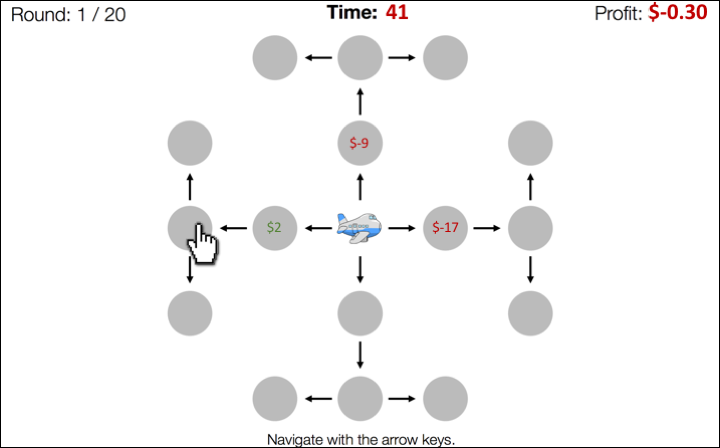
\includegraphics[width=0.49\textwidth]{paradigm_illustration1.png}&
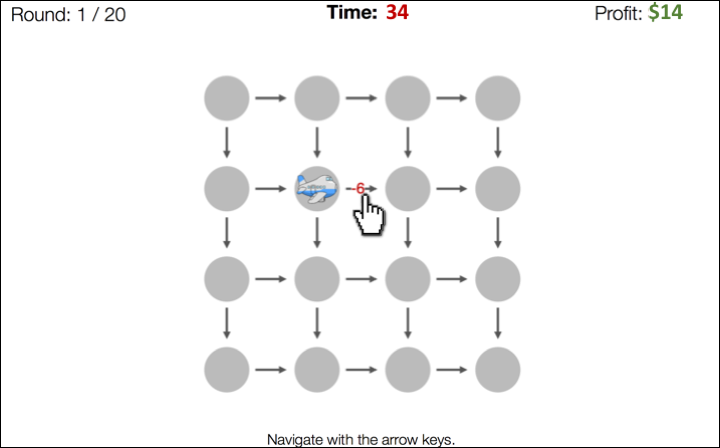
\includegraphics[width=0.49\textwidth]{paradigm_illustration2.png}\\
a) State values revealed with clicks  & b) State values shown while hovering the mouse
\end{tabular}
\caption{Two example paradigms created with the Mouselab-MDP plugin for JsPsych: a) Each state is labeled with the reward for reaching that state; these rewards become visible after they are clicked, with a \$0.10 fee per click. b) The reward for making a transition is revealed only while the mouse is hovering over the corresponding arrow.}
\label{fig:Screenshots}
\end{figure}

% In a given trial, the MDP is first displayed on the screen as a graph (see Figure \ref{fig:Screenshots}). States are positioned according to \texttt{layout} and directed edges are automatically drawn to indicate available actions. State and edge labels are displayed following the parameters discussed above. The participant finds her character in the initial state and navigates through the MDP using the keyboard (the arrow keys by default). The trial ends when the participant reaches a final state (i.e.~one with no available actions).


This novel paradigm offers three advantages over previous behavioral paradigms for the study of planning:
\begin{enumerate}
\item
  The latent cognitive process of planning is made observable by recording the participant's clicks. This allows the experimenter to test hypotheses that would otherwise be difficult to confirm or refute based on overt behavior.
\item
  A wide variety of state-transition and reward structures can be
  displayed automatically. This allows an experimenter to create a large number of highly variable stimuli (potentially automatically with a computer program) in relatively little time (compared to using an image-editing software).  
\item
  The paradigm is packaged as a JsPsych plugin with a concise, yet
  flexible stimuli specification. This allows experimenters with
  only basic knowledge of Javascript to use our plugin to create
  a wide range of qualitatively novel experiments that can be run
  online with crowd-sourcing services such as Amazon Mechanical Turk.
\end{enumerate}


\section{Revealing Planning Strategies}
Here, we present a proof-of-concept case study to illustrate the utility of the Mouselab-MDP paradigm. The data from this experiment sheds new light on the well-studied notion of pruning \cite{Huys2012}.

\subsection{Methods}
We used the Mouselab-MDP plugin for JsPsych. In each trial participants route an airplane from the center of the screen to one of eight final destinations via two intermediate locations (see Figure \ref{fig:Screenshots}a). We specified \texttt{stateLabels} as the rewards associated with the edge leading to each state. We set \texttt{stateDisplay} to `click' and `stateClickCost' to 0.10; thus participants could click on a state to reveal the reward for traveling to that state, at the price of $\$0.10$. Participants were required to spend at least $45$ seconds on every trial to prevent time cost from discouraging participants from clicking and planning. 

We recruited 31 participants on Amazon Mechanical Turk. The task took $31$ minutes on average and participants were paid $\$1.50$ plus a bonus equal to $5\%$ of their earnings on one randomly selected trial (average bonus: $\$1.69$). Participants completed a total of 20 trials in randomized order. The trials differed only in rewards. All rewards were integers between $-\$20$ and $+\$18$ (mean: $4.2$, SD: $10.3$).  The reward functions were designed so that 3-step planning with full information led to significantly higher returns than 2-step planning, 1-step planning, or random choice ($\$38.35$ vs. $\$16.06$--$\$18.30$).


\subsection{Results}

% \begin{enumerate}
% \item{Click frequencies by location}
% \item{Frequent click sequences: \fl{I think this would be most compelling if we find something interesting.}}
% \item{Contingency of click sequence on sampled reward: Is there evidence for pruning?}
% \end{enumerate}

% \begin{figure}
% \includegraphics[width=0.49\textwidth]{results.png}
% \caption{Planning strategies discovered with the Mouselab-planning paradigm illustrated in Figure \ref{fig:Screenshots}a.}
% \label{fig:Results}
% \end{figure}

Figure \ref{fig:click_patterns}a shows the frequency with which participants inspected each of the sixteen states of the task environment (Figure \ref{fig:Screenshots}a) prior to selecting the first flight, in four of the 20 MDPs. Each MDP corresponds to a decision tree with four branches each of which comprises a stem and three outer nodes. Examining Figure \ref{fig:click_patterns}a (and similar plots for all the MDPs), the frequency with which participants inspected the outer nodes of a branch appears to increase with the reward at the stem of the branch. Conversely, participants were less likely to inspect the outer nodes of a branch when its inner node was a large loss. This is indicative of pruning. To quantify this intuitive result, we define pruning as inspecting none of the subsequent nodes of a branch after inspecting the stem. Figure \ref{fig:pruning} shows that the probability with which people prune a branch of their decision tree increases gradually with the magnitude of the loss at its stem. A logistic regression analysis accounting for individual differences in the base rate of pruning confirmed that the increase in pruning with the decrease of the reward at the stem of the branch was statistically significant ($t(1276)=-2.01,p<0.05$). To our knowledge, this is the first analysis to find that pruning changes gradually with the magnitude of the loss or gain.

Our results are consistent with those of \citeA{Huys2012} who showed that a model with a ``specific pruning parameter'' (i.e. a larger discount $\gamma$ applied to states after a large loss) fit participant choices better than a model without such a parameter.
However, their data and model are also consistent with an alternative explanation: people may consider all branches of the tree but discount distant rewards while overweighting immediate losses \cite{Green2004}.
Our data, in contrast, provide direct evidence that participants did not consider states after costly transitions.
This indicates that the continuous discounting parameter of \citeA{Huys2012} may have captured the average effect of many discrete pruning decisions.


% \begin{figure}
% 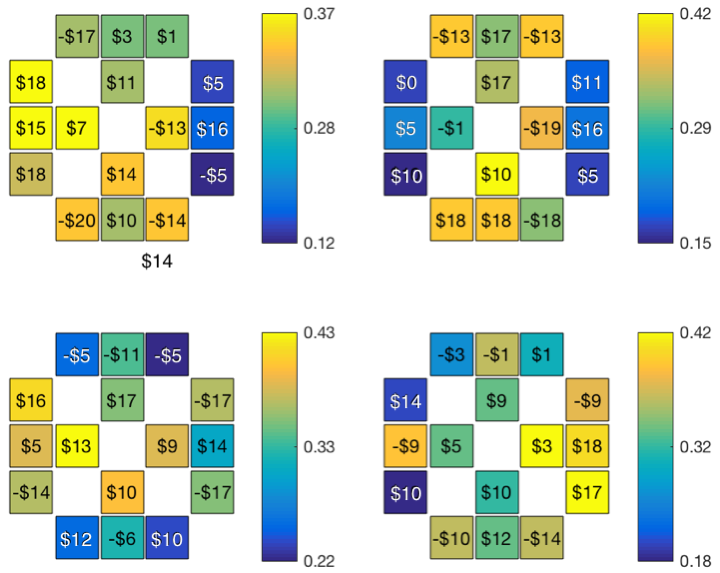
\includegraphics[width=0.99\textwidth]{click_locations_noFB_before1stFlight_small.png}
% \caption{Frequency of sampling by location, across twenty trials. Each subplot shows the location and monetary value of each state for a single trial type. The colors indicate how often each state was inspected before the first move. %\pmk{should we highlight the most common final destination?}
% }  %\fl{I think this would be informative.}
% \label{fig:click_frequencies}
% \end{figure}

\begin{figure}
\begin{tabular}{cc}
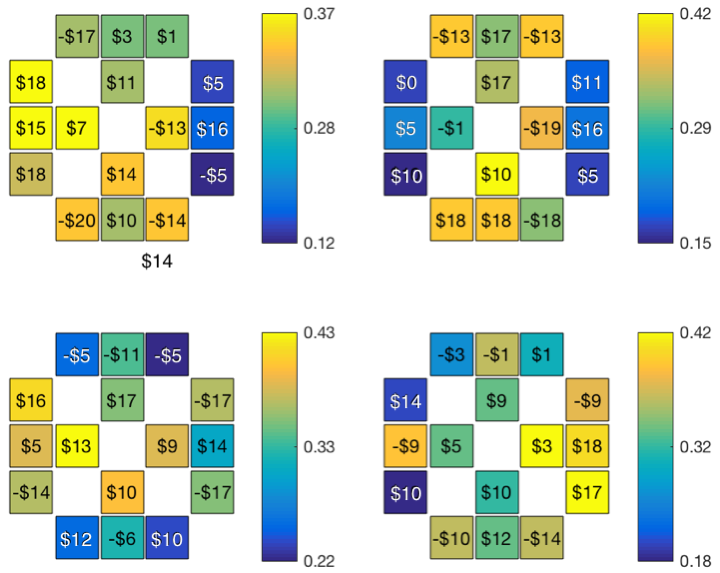
\includegraphics[width=0.49\textwidth]{click_locations_noFB_before1stFlight_small.png}&
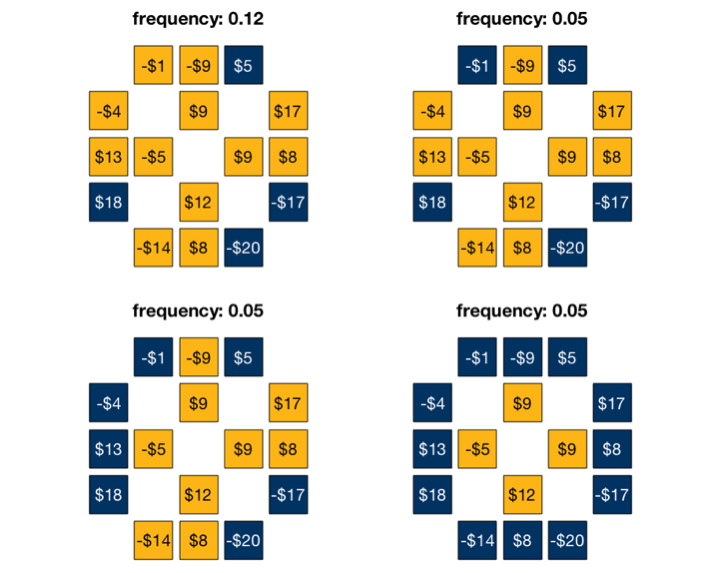
\includegraphics[width=0.49\textwidth]{click_sets_trial4_noFB_small.png}\\
a) Frequency of sampling by location, across four MDPs.  & b) The four most common sets of clicks for one MDP.
\end{tabular}
\caption{Patterns of mouse clicking in humans. a) Each subplot shows the location and monetary value of each state for a different MDP. The colors indicate how often each state was inspected before the first move. b) Frequencies indicate the portion of participants who selected each set, for one particular MDP. Inspected states are gold. The monetary values indicate the reward for flying to that state.}
\label{fig:click_patterns}
\end{figure}

\begin{figure}
\floatbox[{\capbeside\thisfloatsetup{capbesideposition={right,center},capbesidewidth=0cm}}]{figure}[\FBwidth]
{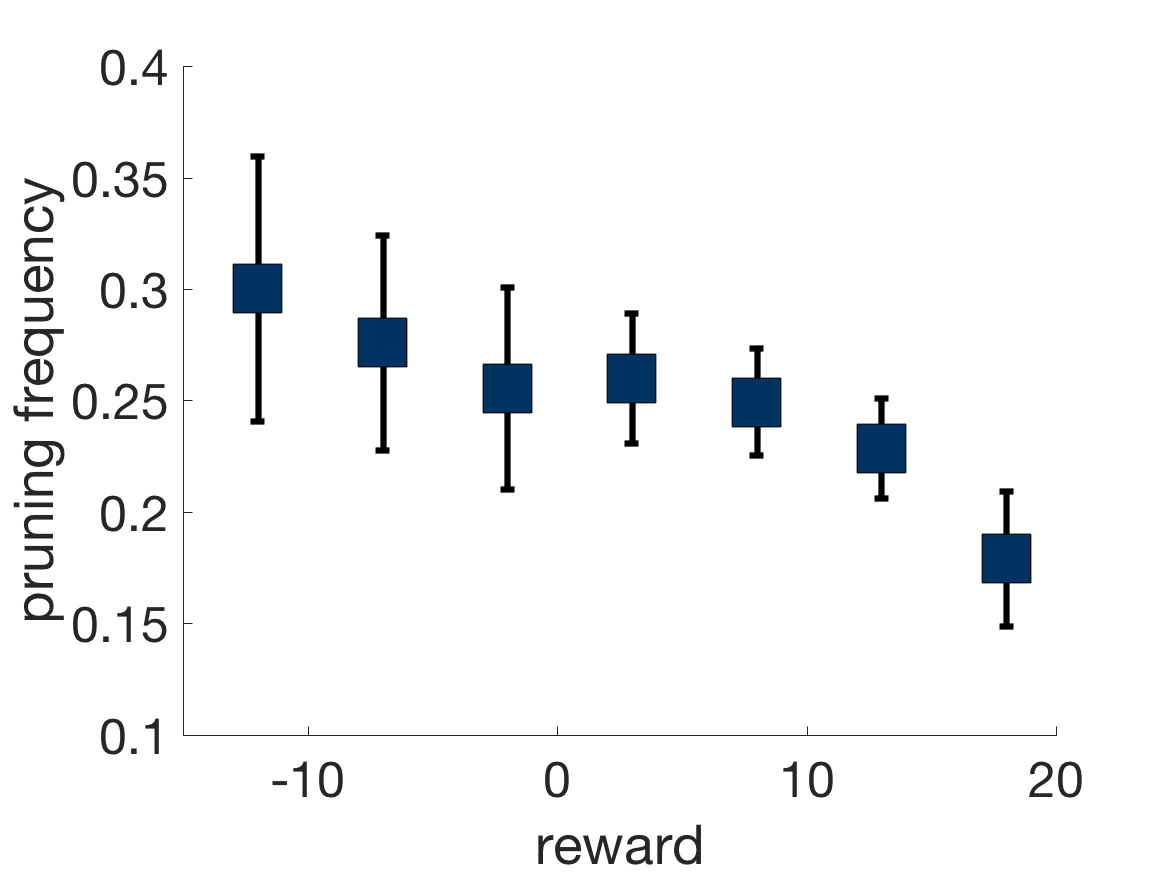
\includegraphics[width=0.45\textwidth]{prunning_any_noFB.png}}
{\caption{Frequency of pruning $\pm 1 \text{SEM}$ (vertical axis) given the reward at the stem of the branch (horizontal axis). Pruning was defined as inspecting none of a branch's outer states (before the second move) after having inspected the reward at its stem (before the first move). Each point shows the mean frequency of pruning.} \label{fig:pruning}}
\end{figure}

Figure \ref{fig:click_patterns}b shows the four most common sets of clicks (before the first flight) for a one MDP. The most frequent strategy inspected exactly one complete path on each of the four branches, and the second most common strategy pruned one or more branches whose reward at the stem was lowest. 

%along with the frequency with which each set of clicks was chosen. %The gold boxes indicate sampled states and the blue boxes indicate unsampled states.\fl{I think we should add a few sentences to characterize these sequences.}

%Figure \ref{fig:pruning} shows the the frequency with which participants do not sample any of the outer states, given that the inner state leading to them was sampled. These frequencies are plotted as a function of the reward of the inner state. This graded dependency between the values of inner states and the sampling frequency of outer states is consistent with a graded pruning effect \cite{Huys2012}.

% \begin{figure}
% \centering
% \begin{subfigure}{.49\textwidth}
%  \label{fig:click_frequencies}
%  \centering
%   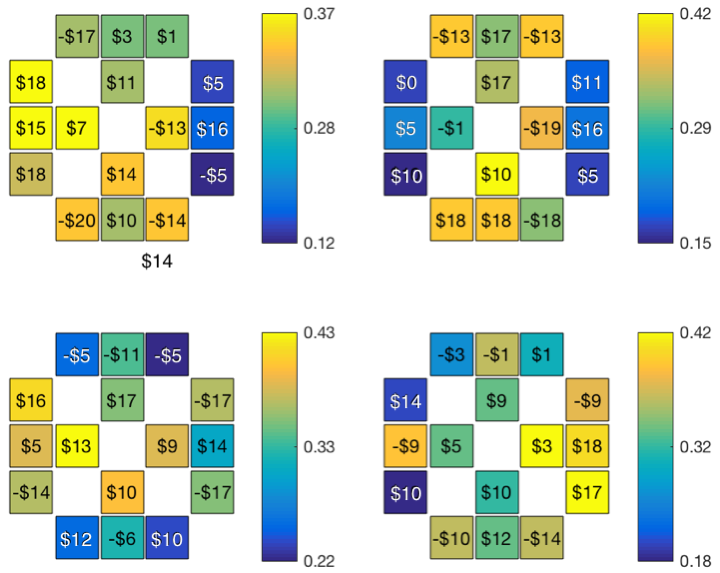
\includegraphics[width=.47\textwidth]{click_locations_noFB_before1stFlight_small.png}
%  \caption{Frequency of sampling by location, across twenty trials. Each subplot shows the location and monetary value of each state for a single trial type. The colors indicate how often each state was inspected before the first move.}
% \end{subfigure}
% \begin{subfigure}{.49\textwidth}
%  \label{fig:click_sets}
%  \centering
%   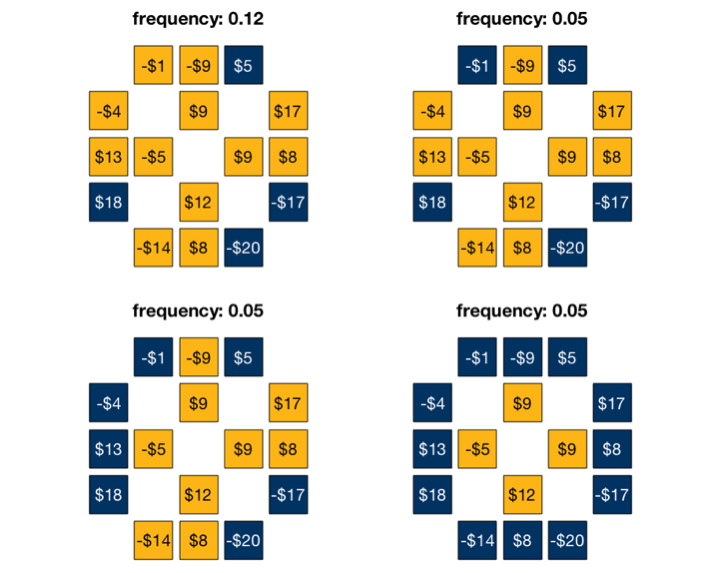
\includegraphics[width=.47\textwidth]{click_sets_trial4_noFB_small.png}
%  \caption{The four most common sets of clicks in two different MDPs (frequencies indicate the portion of participants who selected each set). %Each subplot title indicates the proportion of participants who selected a particular set of clicks.
% Inspected states are gold. The monetary values indicate the reward for flying to that state. %\pmk{should we highlight the most common final destination here?}}
% \end{subfigure}
% \caption{Patterns of observation in humans.}
% \label{fig:human_data}
% \end{figure}

\section{Conclusion}
We have developed a process-tracing paradigm for the study of planning and demonstrated that it can reveal the processes of planning at a higher level of resolution than standard behavioral paradigms. We showed that the paradigm provides a new look at one aspect of planning: pruning. However, many questions remain. Do people plan in a breadth-first or depth-first fashion? Do they plan and then act all at once, or do they interleave planning and acting? How do they balance the cost of planning with the potential for increased reward? Do these aspect of planning vary based on the problem structure? If so, how do people meta-reason about what planning strategies to employ? How do people learn and refine their planning strategies? How and why do people differ in their planning abilities?  No single paradigm can give an answer to all these questions. However, Mouselab-MDP can produce data that speaks to all of them.

Future work will extend the Mouselab-MDP plugin to stochastic environments and enable tracing additional aspects of the planning process, including representation of a transition model and heuristic evaluation of state values.

% We have developed a process-tracing paradigm for the study of planning and demonstrated that it can reveal the processes of planning at a higher level of resolution than standard behavioral paradigms. We showed that the paradigm provides a new look at one aspect of planning: pruning. However, many questions remain. Do people adjust their planning strategies based on cost of gathering information and potential for reward? Do people plan in a breadth-first or depth-first fashion; does it depend on the problem structure? Do people typically plan and then act all at once, or do they interleave planning and acting? All of these questions can be answered with data from the Mouselab-MDP paradigm. 

% In general, we hope that this paradigm will facilitate reverse-engineering people's highly efficient planning algorithms evaluating human planning against bounded optimal planning, studying how planning strategies are learned and refined, and investigating how and why they differ between people. 
% Future work will extend the Mouselab-MDP plugin to stochastic environments and enable tracing additional aspects of the planning process such as how people build a mental representation of the state space, the available actions, and how the states are connected by actions. %Future work will leverage the Mouselab-MDP paradigm to study whether and too what extent people's planning mechanisms exhibit the adaptive flexibility that \citeA{Payne1988} observed for multi-alternative risky choice.


\bibliographystyle{apacite}
\renewcommand{\bibliographytypesize}{\small}
\setlength{\bibleftmargin}{.05in}
\setlength{\bibindent}{-\bibleftmargin}
\bibliography{references}


\end{document}